% arara: xelatex: { shell: yes }
% arara: biber
% arara: xelatex: { shell: yes }
% arara: xelatex: { shell: yes }
% arara: xelatex: { shell: yes }

%% This is the ctufit-thesis example file. It is used to produce theses
%% for submission to Czech Technical University, Faculty of Information Technology.
%%
%% Get the newest version from
%% https://gitlab.fit.cvut.cz/theses-templates/FITthesis-LaTeX
%%
%%
%% Copyright 2021, Eliska Sestakova and Ondrej Guth
%%
%% This work may be distributed and/or modified under the
%% conditions of the LaTeX Project Public Licenese, either version 1.3
%% of this license or (at your option) any later version.
%% The latest version of this license is in
%%  https://www.latex-project.org/lppl.txt
%% and version 1.3 or later is part of all distributions of LaTeX
%% version 2005/12/01 or later.
%%
%% This work has the LPPL maintenance status `maintained'.
%%
%% The current maintainer of this work is Ondrej Guth.
%% Contact ondrej.guth@fit.cvut.cz for bug reports.
%% Alternatively, submit bug reports into the tracker at
%% https://gitlab.fit.cvut.cz/theses-templates/FITthesis-LaTeX/issues
%%
%%

%%%%%%%%%%%%%%%%%%%%%%%%%%%%%%%%%%%%%%%%%
% CLASS OPTIONS
% language: czech/english/slovak
% thesis type: bachelor/master/dissertation
%%%%%%%%%%%%%%%%%%%%%%%%%%%%%%%%%%%%%%%%%
\documentclass[czech,bachelor,unicode]{template/ctufit-thesis}

%%%%%%%%%%%%%%%%%%%%%%%%%%%%%%%%%%
% FILL IN THIS INFORMATION
%%%%%%%%%%%%%%%%%%%%%%%%%%%%%%%%%%
\ctufittitle{Webová aplikace pro správu a sdílení receptů} % replace with the title of your thesis
\ctufitauthorfull{Vojtěch Moravec} % replace with your full name (first name(s) and then family name(s) / surname(s)) including academic degrees
\ctufitauthorsurnames{Moravec} % replace with your surname(s) / family name(s)
\ctufitauthorgivennames{Vojtěch} % replace with your first name(s) / given name(s)
\ctufitsupervisor{Ing.\,Oldřich Malec} % replace with name of your supervisor/advisor (include academic degrees)
\ctufitdepartment{Katedra softwarového inženýrství} % replace with the department of your defence
\ctufityear{2022} % replace with the year of your defence
\ctufitdeclarationplace{Praze} % replace with the place where you sign the declaration
\ctufitdeclarationdate{\today} % replace with the date of signature of the declaration
\ctufitabstractCZE{Fill in abstract of this thesis in Czech language. Class aptent taciti sociosqu ad litora torquent per conubia nostra, per inceptos hymenaeos. Cras pede libero, dapibus nec, pretium sit amet, tempor quis. Sed vel lectus. Donec odio tempus molestie, porttitor ut, iaculis quis, sem. Suspendisse sagittis ultrices augue.}
\ctufitabstractENG{Fill in abstract of this thesis in English language. Class aptent taciti sociosqu ad litora torquent per conubia nostra, per inceptos hymenaeos. Cras pede libero, dapibus nec, pretium sit amet, tempor quis. Sed vel lectus. Donec odio tempus molestie, porttitor ut, iaculis quis, sem. Suspendisse sagittis ultrices augue.}
\ctufitkeywordsCZE{frontend, Vue, Vuetify, recepty na vaření, webová aplikace, serverless, Firebase} % TODO: Specifikovat recepty.
\ctufitkeywordsENG{frontend, Vue, Vuetify, recipes, web app, serverless, Firebase}
%%%%%%%%%%%%%%%%%%%%%%%%%%%%%%%%%%
% END FILL IN
%%%%%%%%%%%%%%%%%%%%%%%%%%%%%%%%%%

%%%%%%%%%%%%%%%%%%%%%%%%%%%%%%%%%%
% CUSTOMIZATION of this template
% Skip this part or alter it if you know what you are doing.
%%%%%%%%%%%%%%%%%%%%%%%%%%%%%%%%%%

\RequirePackage{iftex}[2020/03/06]
\iftutex % XeLaTeX and LuaLaTeX
    \RequirePackage{ellipsis}[2020/05/22] %ellipsis workaround for XeLaTeX
\else
    \RequirePackage[utf8]{inputenc}[2018/08/11] %this file encoding
    \RequirePackage{lmodern}[2009/10/30] % vector flavor of Computer Modern font
\fi

% hyperlinks
\RequirePackage[pdfpagelayout=TwoPageRight,colorlinks=false,allcolors=decoration,pdfborder={0 0 0.1}]{hyperref}[2020-05-15]

% uncomment the following to hide all hyperlinks
% \RequirePackage[pdfpagelayout=TwoPageRight,hidelinks]{hyperref}[2020-05-15]

\RequirePackage{pdfpages}[2020/01/28]

\setcounter{secnumdepth}{4} % numbering sections; 4: subsubsection



%%%%%%%%%%%%%%%%%%%%%%%%%%%%%%%%%%
% CUSTOMIZATION of this template END
%%%%%%%%%%%%%%%%%%%%%%%%%%%%%%%%%%


%%%%%%%%%%%%%%%%%%%%%%
% DEMO CONTENTS SETTINGS
% You may choose to modify this part.
%%%%%%%%%%%%%%%%%%%%%%
\usepackage{dirtree}
\usepackage{lipsum,tikz}
\usepackage{csquotes}
\addbibresource{text/bib-database.bib}
%\usepackage{listings} % typesetting of sources
\usepackage{minted} % typesetting of sources

%theorems, definitions, etc.
\theoremstyle{plain}
\newtheorem{theorem}{Věta}
\newtheorem{lemma}[theorem]{Tvrzení}
\newtheorem{corollary}[theorem]{Důsledek}
\newtheorem{proposition}[theorem]{Návrh}
\newtheorem{definition}[theorem]{Definice}
\theoremstyle{definition}
\newtheorem{example}[theorem]{Příklad}
\theoremstyle{remark}
\newtheorem{note}[theorem]{Poznámka}
\newtheorem*{note*}{Poznámka}
\newtheorem{remark}[theorem]{Pozorování}
\newtheorem*{remark*}{Pozorování}
\numberwithin{theorem}{chapter}
%theorems, definitions, etc. END
%%%%%%%%%%%%%%%%%%%%%%
% DEMO CONTENTS SETTINGS END
%%%%%%%%%%%%%%%%%%%%%%

\begin{document}
\frontmatter\frontmatterinit % do not remove these two commands

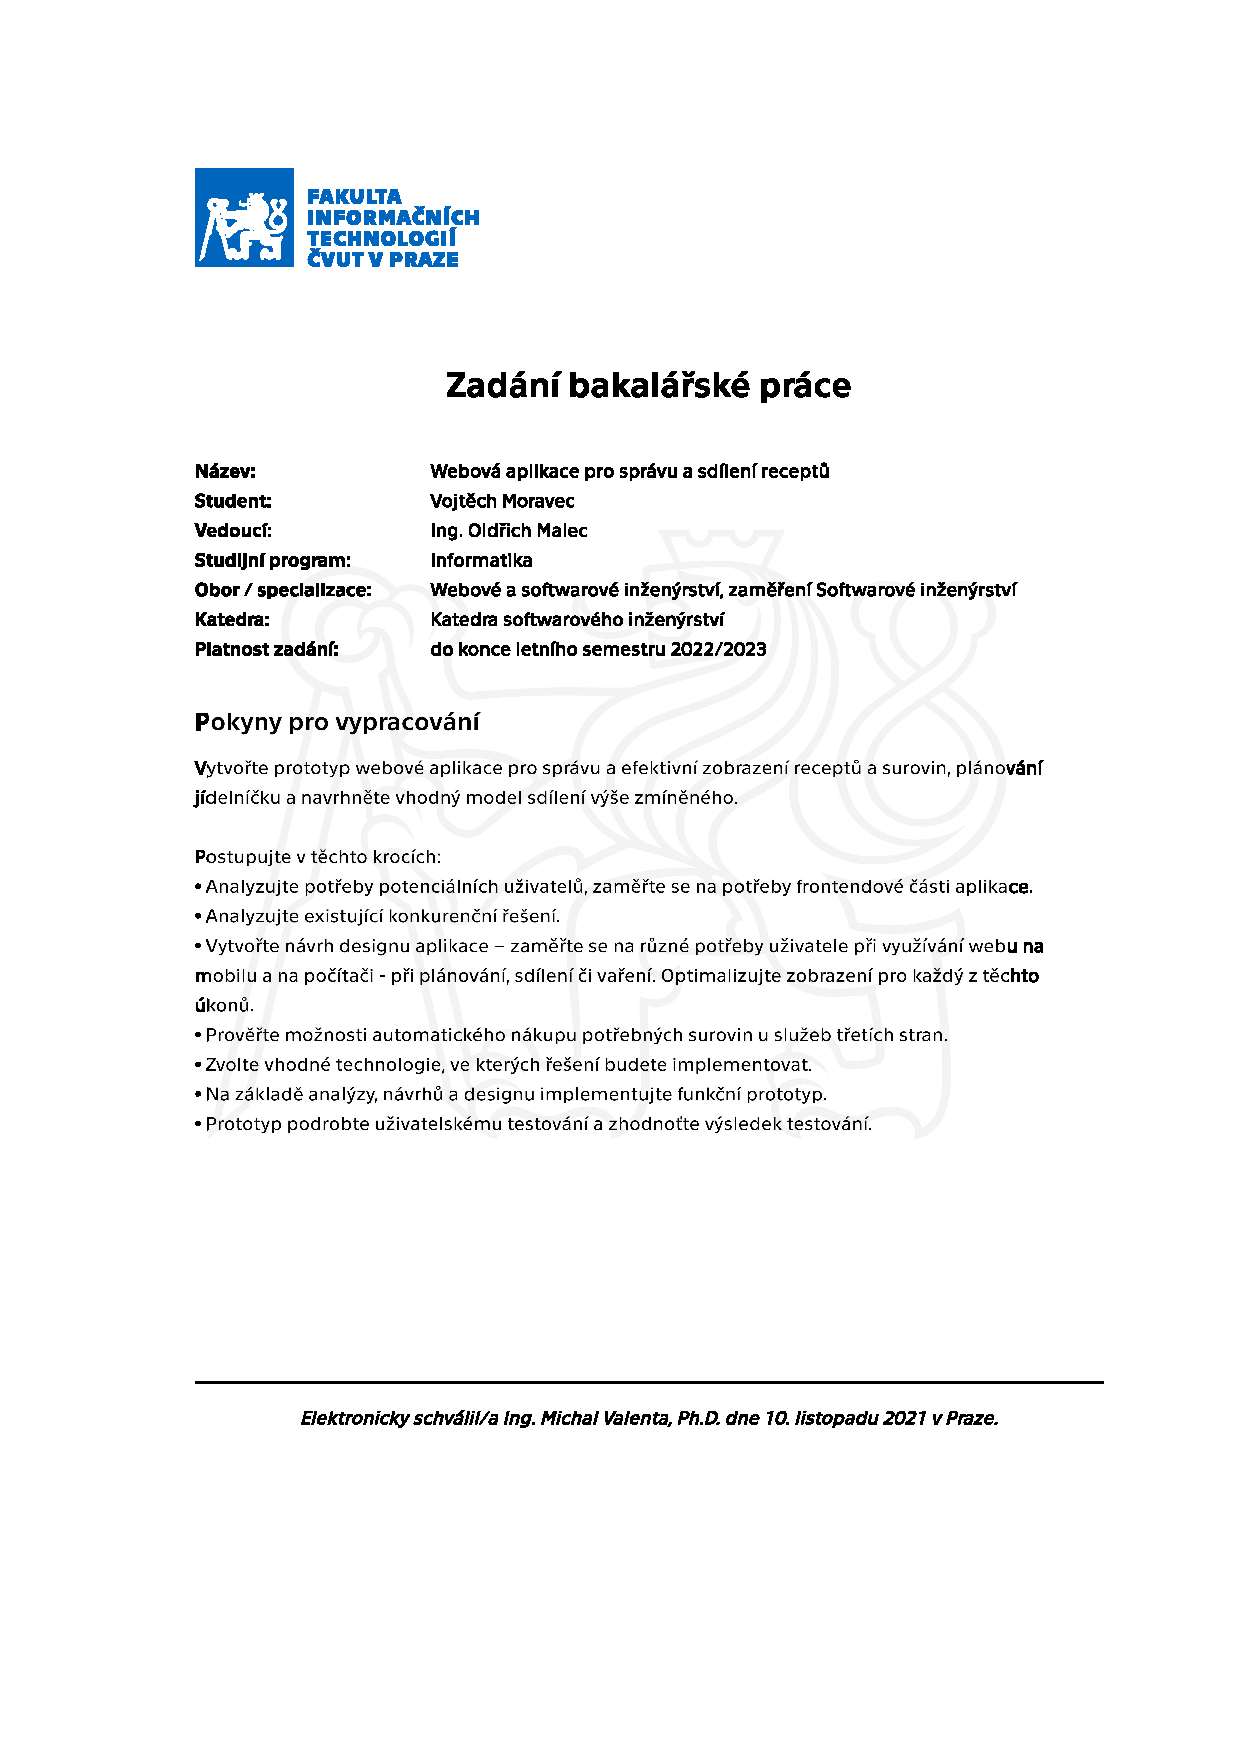
\includepdf{pdf/assignment-include.pdf} % replace that file with your thesis assignment provided by study office

\thispagestyle{empty}\cleardoublepage\maketitle % do not remove these three commands

\imprintpage % do not remove this command

\tableofcontents % do not remove this command
%%%%%%%%%%%%%%%%%%%%%%
% list of other contents: figures, tables, code listings, algorithms, etc.
% add/remove commands accordingly
%%%%%%%%%%%%%%%%%%%%%%
\listoffigures % list of figures
\begingroup
\let\clearpage\relax
\listoftables % list of tables
%\lstlistoflistings % list of source code listings generated by the listings package TODO: Minted switch
\listoflistings % list of source code listings generated by the minted package
\endgroup
%%%%%%%%%%%%%%%%%%%%%%
% list of other contents END
%%%%%%%%%%%%%%%%%%%%%%

%%%%%%%%%%%%%%%%%%%
% ACKNOWLEDGMENT
% FILL IN / MODIFY
% This is a place to thank people for helping you. It is common to thank your supervisor.
%%%%%%%%%%%%%%%%%%%
\begin{acknowledgmentpage}
	Chtěl bych poděkovat především sit amet, consectetuer adipiscing elit. Curabitur sagittis hendrerit ante. Class aptent taciti sociosqu ad litora torquent per conubia nostra, per inceptos hymenaeos. Cras pede libero, dapibus nec, pretium sit amet, tempor quis. Sed vel lectus. Donec odio tempus molestie, porttitor ut, iaculis quis, sem. Suspendisse sagittis ultrices augue.
\end{acknowledgmentpage}
%%%%%%%%%%%%%%%%%%%
% ACKNOWLEDGMENT END
%%%%%%%%%%%%%%%%%%%


%%%%%%%%%%%%%%%%%%%
% DECLARATION
% FILL IN / MODIFY
%%%%%%%%%%%%%%%%%%%
% INSTRUCTIONS
% ENG: choose one of approved texts of the declaration. DO NOT CREATE YOUR OWN. Find the approved texts at https://courses.fit.cvut.cz/SFE/download/index.html#_documents (document Declaration for FT in English)
% CZE/SLO: Vyberte jedno z fakultou schvalenych prohlaseni. NEVKLADEJTE VLASTNI TEXT. Schvalena prohlaseni najdete zde: https://courses.fit.cvut.cz/SZZ/dokumenty/index.html#_dokumenty (prohlášení do ZP)
\begin{declarationpage}
    Prohlašuji, že jsem předloženou práci vypracoval samostatně a že jsem uvedl veškeré
    použité informační zdroje v souladu s Metodickým pokynem o dodržování etických
    principů při přípravě vysokoškolských závěrečných prací.

    Beru na vědomí, že se na moji práci vztahují práva a povinnosti vyplývající ze zákona
    č. 121/2000 Sb., autorského zákona, ve znění pozdějších předpisů. V souladu s ust.
    § 2373 odst. 2 zákona č. 89/2012 Sb., občanský zákoník, ve znění pozdějších předpisů,
    tímto uděluji nevýhradní oprávnění (licenci) k užití této mojí práce, a to včetně všech
    počítačových programů, jež jsou její součástí či přílohou a veškeré jejich
    dokumentace (dále souhrnně jen „Dílo“), a to všem osobám, které si přejí Dílo užít.
    Tyto osoby jsou oprávněny Dílo užít jakýmkoli způsobem, který nesnižuje hodnotu
    Díla, avšak pouze k nevýdělečným účelům. Toto oprávnění je časově, teritoriálně
    i množstevně neomezené.
\end{declarationpage}
%%%%%%%%%%%%%%%%%%%
% DECLARATION END
%%%%%%%%%%%%%%%%%%%

\printabstractpage % do not remove this command

%%%%%%%%%%%%%%%%%%%
% SUMMARY
% FILL IN / MODIFY
% OR REMOVE ENTIRELY (upon agreement with your supervisor)
% (appropriate to remove in most theses)
%%%%%%%%%%%%%%%%%%%
\begin{summarypage}
\section*{Summary section}

\lipsum[1][1-8]

\section*{Summary section}

\lipsum[2][1-6]

\section*{Summary section}

\lipsum[3]

\section*{Summary section}

\lipsum[2]

\section*{Summary section}

\lipsum[1][1-8] Lorem lorem lorem.
\end{summarypage}
%%%%%%%%%%%%%%%%%%%
% SUMMARY END
%%%%%%%%%%%%%%%%%%%

%%%%%%%%%%%%%%%%%%%
% ABBREVIATIONS
% FILL IN / MODIFY
% OR REMOVE ENTIRELY
% List the abbreviations in lexicography order.
%%%%%%%%%%%%%%%%%%%
%! Author = vojmo
%! Date = 15.11.2021

\chapter{Seznam zkratek}

\begin{tabular}{rl}
    API & Application Programming Interface \\
    SQL & Structured Query Language \\
    NoSQL & Not Only SQL \\
    JSON & JavaScript Object Notation \\
    FE & Frontend \\
    NPM & Node Package Manager \\
    CLI & Command Line Interface \\
    YML & Yaml Ain't Markup Language \\
    JS & JavaScript \\
    PWA & Progressive Web App \\
    CSS & Cascading Style Sheets \\
\end{tabular}

%%%%%%%%%%%%%%%%%%%
% ABBREVIATIONS END
%%%%%%%%%%%%%%%%%%%

\mainmatter\mainmatterinit % do not remove these two commands

%%%%%%%%%%%%%%%%%%%
% THE THESIS
% MODIFY ANYTHING BELOW THIS LINE
%%%%%%%%%%%%%%%%%%%

%! Author = Vojta
%! Date = 21.10.2021

\chapter{Úvod}

Vaření se týká spousty lidí. Mladší generace k tomu používá recepty, které jsou dostupné na internetu. Recepty, které najdou
a které se jim osvědčí, jsou často na jiných stránkách a správa těchto receptů se stává nereálná. Na druhou stranu na nejznámějších
portálech není možné si recepty ukládat soukromně a tak spoustu starších lidí nevyužije možnosti digitalizace jejich receptů.
Většina z nich si totiž uchovává své recepty napsané na listech papíru, což ale v dnešní době již není praktické řešení. Už jen kvůli
sdílení receptu s někým, kdo si ho vyžádá, což je celkem běžná záležitost.

Výsledek této práce bude moci použít široká veřejnost -- každý kdo vaří podle receptů. Aplikace jim pomůže s jednoduchým
zadání receptů do sbírky, kde mohou mít všechny recepty na jednom místě. Dále budou moci uživatelé využít plánovače, kam
lze zanést již přidané recepty či počet porcí. Pokud nejsou zvyklí plánovat a spíše řeší věci na poslední chvíli, bude
pro ně připraven rychlý návrh receptu. V neposlední řadě bude jednoduché své recepty sdílet s ostatními uživateli.

V práci popisuji proces vývoje webové aplikace od analýzy přes návrh až po implementaci. Zaměřím se hlavně na frontend v
javascriptovém frameworku Vue.js, ale provedu čtenáře i backendovou částí, která je tvořena pomocí nástrojem Firebase od
společnosti Google. Začnu sběrem informací od potencionálních uživatelů, pomocí kterých sestavím funkční a nefunkční požadavky.
Poté zanalyzuji konkurenční řešení a popíšu jejich plusy či nevýhody. Poté představím technologie, které jsem si vybral pro
vývoj. Dále navrhnu uživatelské rozhraní, grafické prvky či datovou strukturu aplikace. Na základě předchozích kapitol implementuji
aplikaci a zmíním problémy, se kterými jsem se při vývoji setkal. Sestavím test pro uživatele a zhodnotím jeho výsledky.
Na závěr zmíním funkce které jsem nestihl implementovat či rozšíření, která by se v budoucnosti hodila.

Téma mě zaujalo, protože si myslím, že nabízí spoustu míst, pro učení se nových věcí. Také jsem nenašel žádnou alternativu,
která by nabízela všechny funkce, které moje řešení poskytuje.

\chapter{Cíl}
% TODO: Vylepšit
Cílem této bakalářské práce je vytvořit prototyp webové aplikace pro správu receptů. Dále je nutné prozkoumat možnosti
zjednodušení nákupu surovin či plánování vaření jídel.

Nejdříve zanalyzuji potřeby potenciálních uživatelů, kde se pokusím zjistit, které všechny funkce by ocenili. Poté se
zaměřím na existující řešení, která porovnám s mým řešením a popíšu vylepšení.

Dále vytvořím návrh designu aplikace -- wireframy, které zachycují zároveň, jak aplikace vypadá. Důraz kladu na rozdíly
mezi použitím na mobilu a počítači.

Na základě analýzy a návrhu vyberu technologie, které použiju pro implementaci funkčního prototypu.

Na konec podrobím aplikaci uživatelskému testování a zhodnotím jeho výsledky.

%! Author = Vojta
%! Date = 21.10.2021

\chapter{Analýza}

\section{Kvalitativní průzkum}

%! Author = Vojta
%! Date = 21.10.2021

\chapter{Technologie}

\section{Výběr}
Vzhledem k tomu, že aplikace byla původně zamýšlena jako osobní projekt, který by si následně spravoval sám vedoucí a já
jsem měl zkušenosti pouze s frameworkem Vue.js, hlavní technologie, okolo které se projekt postaví, byla předem daná. Poté
jsem postupně vybíral další součásti, které bychom mohli využít. Velkou výhodou bylo, že právě vedoucí práce má s většinou
z těchto knihoven či pluginů zkušenosti, a tak když se mi něco nedařilo, mohl jsem se na něj obrátit.

\section{Vue.js}
Vue je progresivní JavaScriptový framework, který narozdíl od konkurenčních řešení (React, Angular) nezaštiťuje žádná velká
korporace, ale je vyvíjen komunitou.\cite{VueJS} Zvolil jsem verzi 3, protože je to lepší řešení do budoucna, než později aktualizovat
celou aplikaci z verze 2. V pozdější fázi vývoje se ale ukázalo, že pro verzi 3 nebyla plně dokončena hlavní knihovna, kterou jsem chtěl využít.
Musel jsem tak ponížit verze všech závislostí a přejít tak na verzi 2.

\section{Vuetify}
Vuetify je knihovna implementující různé komponenty, které je možné použít při tvorbě uživatelského rozhraní. Kromě toho
usnadňuje práci s rozložením na stránce, přizpůsobením barevného téma, ikonami atd. Další výhodou jsou týdenní aktualizace
momentální verze, které přidávají nové funkce a opravují nalezené chyby.\cite{VuetifyWhy}
Bohužel tato knihovna nebyla v době vývoje plně dokončena a byla pouze v alpha verzi, tudíž spoustu věci nefungovalo jak by mělo.

\section{Vuex}
Knihovna Vuex~\cite{Vuex} se využívá pro uložení stavu aplikace. Je vhodné ji využít u dat, která jsou využívána na více místech a jejich
předávání skrz komponenty by bylo jinak složité.

Změna či přístup k stavu a všechny operace nad ním se řeší ve speciálním souboru, kde se Vuex inicializuje. K těmto operacím využijeme \emph{state, mutations, getters, actions a modules}.
\emph{State} označuje strukturu dat, tedy pokud potřebuji nějak zaznamenávat recepty, vytvořím zde pole či objekt a s ním dále pracuji. Pro to abych přidal recept využiji \emph{actions} v kombinaci s
\emph{mutations}. \emph{Actions} je obal funkcí, které můžu zavolat odkudkoliv z aplikace a ty provedou nějakou změnu nad daty. Například data stáhnou, aktualizují nebo nastaví hodnotu, kterou uživatel
zadá. Mutations poté vyvoláme pomocí funkce \mintinline{js}|commit|. Té předáme název mutace, která se má zavolat a tzv. \emph{payload}, tedy data, která chceme do stavu zapsat. Mutace již poté pouze zapíše
do stavu a nic dalšího by řešit neměla.

Pro získání stavu lze využít \emph{getters}. V těchto funkcích by také neměla být žádná další logika, ačkoliv se zde dá vytvořit drobné filtrování či řazení.
Když se aplikace rozroste a obsahuje mnoho dat, tak aby všechny tyto části byly přehledné, je možné vytvořit více modulů a spravovat data která mají něco společného
odděleně. Samotné moduly se pak naimportují do \emph{modules} a jsou přístupné v celé aplikaci.

\section{Vue i18n}
I18n~\cite{i18n} je rozšíření pro překlady, díky kterému je možné texty v aplikaci napsat v několika jazycích. Nejprve jsem tvořil aplikaci dvojjazyčně
v angličtině a čestině, ale nakonec jsem se rozhodl, že prozatím dává aplikace smysl pouze v češtině. Nicméně překlady jsem ponechal a v budoucnu
je možné je využít.

\section{Firebase}
Firebase~\cite{Firebase} je platforma pro vývoj aplikací. Nabízí spoustu produktů, které je možné využít a tím zjednodušit vývoj.
Dané produkty mohou mezi sebou komunikovat a reagovat na různé události. Firebase poskytuje multiplatformní SDK, což znamená, že je
možné vyvíjet v několika programovacích jazycích jako je Java, Kotlin, Swift, JavaScript nebo C++. V kombinaci s touto platformou je možné
využít další nástroje od společnosti Google, jako jsou Analytics, Google Ads a další. K tomu lze přidat rozšíření, které vyžadují jen základní
konfiguraci a propojí aplikaci s dalšími externími systémy, jako je Stripe~\cite{Stripe} či Algolia~\cite{Algolia}.

\subsection{Ceny}
Firebase má velikou výhodu v tom, že je zdarma, pokud uživatelé nevyčerpají určitý objem dat či přístupů k databázi. Tato kapacita se resetuje
denně nebo měsíčně, podle toho o jaký podsystém se jedná. V nabídce jsou dva plány. První \emph{Spark Plan} je úplně zadarmo, ale má určitá omezení.
Na druhou stranu \emph{Blaze Plan} má stejné limity a platí se pouze za jejich překročení. Tedy například pro databázi Firestore je zdarma padesát tisíc
čtení denně pro oba plány a pro \emph{Blaze Plan} poté stojí každých dalších sto tisíc čtení 1,40 Kč.~\cite{FirebasePricing}

\subsection{Firestore}
Cloud Firestore~\cite{Firestore} je NoSQL dokumentová databáze. Narozdíl od SQL databází, které se soustředí na snížení duplikace dat, se dokumentová
databáze zaměruje na časté aktualizace a změny. Největší rozdíl mezi těmito typy je způsob uložení dat. SQL reprezentuje data pomocí
tabulek s řádky a sloupci, dokumentová databáze má JSON dokumenty a jejich kolekce. To vede k flexibilnějšímu datovému modelu, rychlejším
dotazům a lehčímu vývoji pro vývojáře.~\cite{MongoDBNoSQL}

Firestore nabízí vlastní řešení bezpečnosti přes Firebase Rules, které více přiblížím v kapitole o implementaci pomocí ukázek.

\subsection{Storage}
Cloud Storage je uložiště, kam je možné ukládat různé soubory, které uživatelé poutřebují při používání aplikace. V mém případě to
budou fotografie jídel či surovin. Pro ukládání dat se používají takzvané \emph{Cloud Storage buckets}, což jsou pouze kontejnery,
které můžeme využít tak, aby data byla organizovaná~\cite{FirebaseBucket}. K tomu lze vytvořit vnitřní strukturu pomocí složek nebo
data oddělit podle jejich provázanosti do různých kontejnerů.

\subsection{Hosting}
Webová aplikace musí být někde dostupná, aby k ní uživatelé mohli přistoupit. K tomu lze v rámci Firebase využít \emph{Hosting}.
Ten nabízí rychlé SSD disky, na kterých web běží, SSL certifikáty pro vlastní domény zdarma, jednoduchý \emph{deploy} nebo náhledy
aplikace předtím než je nasazena na produkci.~\cite{FirebaseHosting}

\subsection{Functions}
Firebase Cloud Functions mají za úkol vývojářům ulehčit vývoj backendu tak, aby nemuseli řešit záležitosti okolo správy serverů.
Funkce, které na tomto systému běží mohou reagovat na širokou škálu událostí uvnitř Firebase produktů. Například pokud se do aplikace
přihlásí nový uživatel, může se spustit funkce, která mu odešle uvítací email. Jako programovací jazyk se pro psaní funkcí použivá Node.js.~\cite{FirebaseFunctions}

\section{Fulltextové vyhledávání}
Při práci s Firebase jsem zjistil, že při dotazování se na záznamy není možné filtrovat podle názvu
(abych byl přesný, možné to je, ale není to vhodné). Po zkoumání dokumentace, jsem našel stránku s doporučením pro
fulltextové hledání. V nabídce byla tři řešení.~\cite{FulltextSearch}

\begin{itemize}
    \item Elastic
    \item Algolia
    \item Typesense
\end{itemize}

Problém jsem řešil s vedoucím a přišli jsme na několik možných řešení sami. Stáhnout si data o všech receptech ve formátu
\emph{id:name} a poté filtrovat výsledky hledání na FE. Dále bychom mohli použít Firebase Cloud Functions, kde bychom
využili hashování. Nakonec jsem se ale rozhodl, že využiji jedno z nabízených řešení přímo Googlem.

Vybral jsem Algolii~\cite{Algolia}, kvůli dobré podpoře Vue a Firebase, nejmenší složitosti implementace a bezplatnému základnímu plánu.

Při vývoji jsem ale zjistil, že základní režim (tedy 10 000 čtení za měsíc) nejspíše stačit nebude. Nakonec jsem proto přešel na
frontendové vyhledávání. Všechna data jsem stáhnul při načtení aplikace a poté s nimi dál pracoval.

\section{Vue Router} % TODO: Více rozepsat
V aplikaci je potřeba mít navigaci. Ve Vue se používá Vue Router~\cite{VueRouter}, který umožní pohyb po různých stránkách.

\subsection{SPA}
SPA neboli \emph{single page application} je stránka, která využívá takové architektury, kde použitá technologie nejen kontroluje
vzhled stránky, ale i data a manipulaci s nimi a navigaci tím způsobem, že není nutné provádět obnovení stránky.\cite{VueSPA}

Pro demonstraci rozdílu mezi MPA a SPA jsem zvolil následující diagramy.

\begin{figure}[H]
    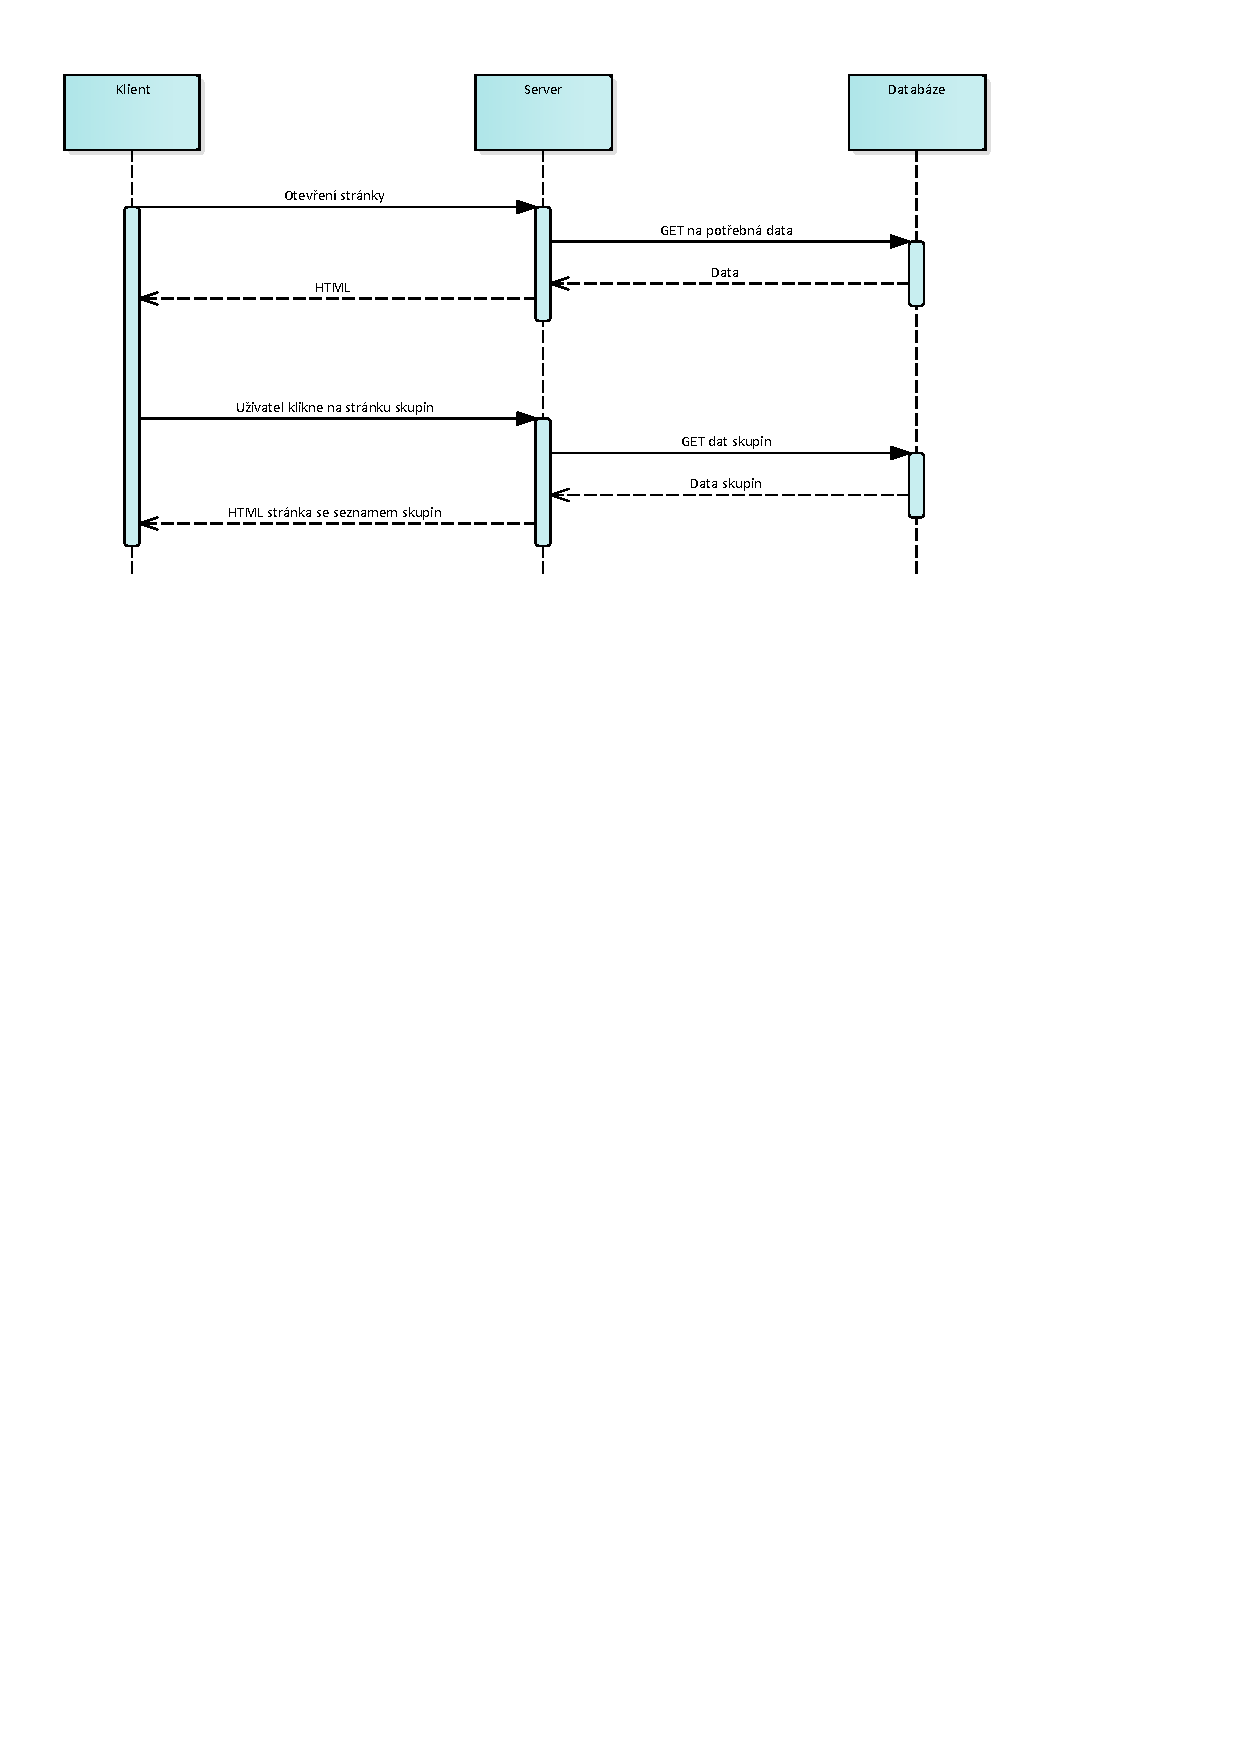
\includegraphics[width=\textwidth]{pdf/MPA-model}
    \caption{MPA Model} \label{picture:recipeo:mpa-model}
\end{figure}
\begin{figure}[H]
    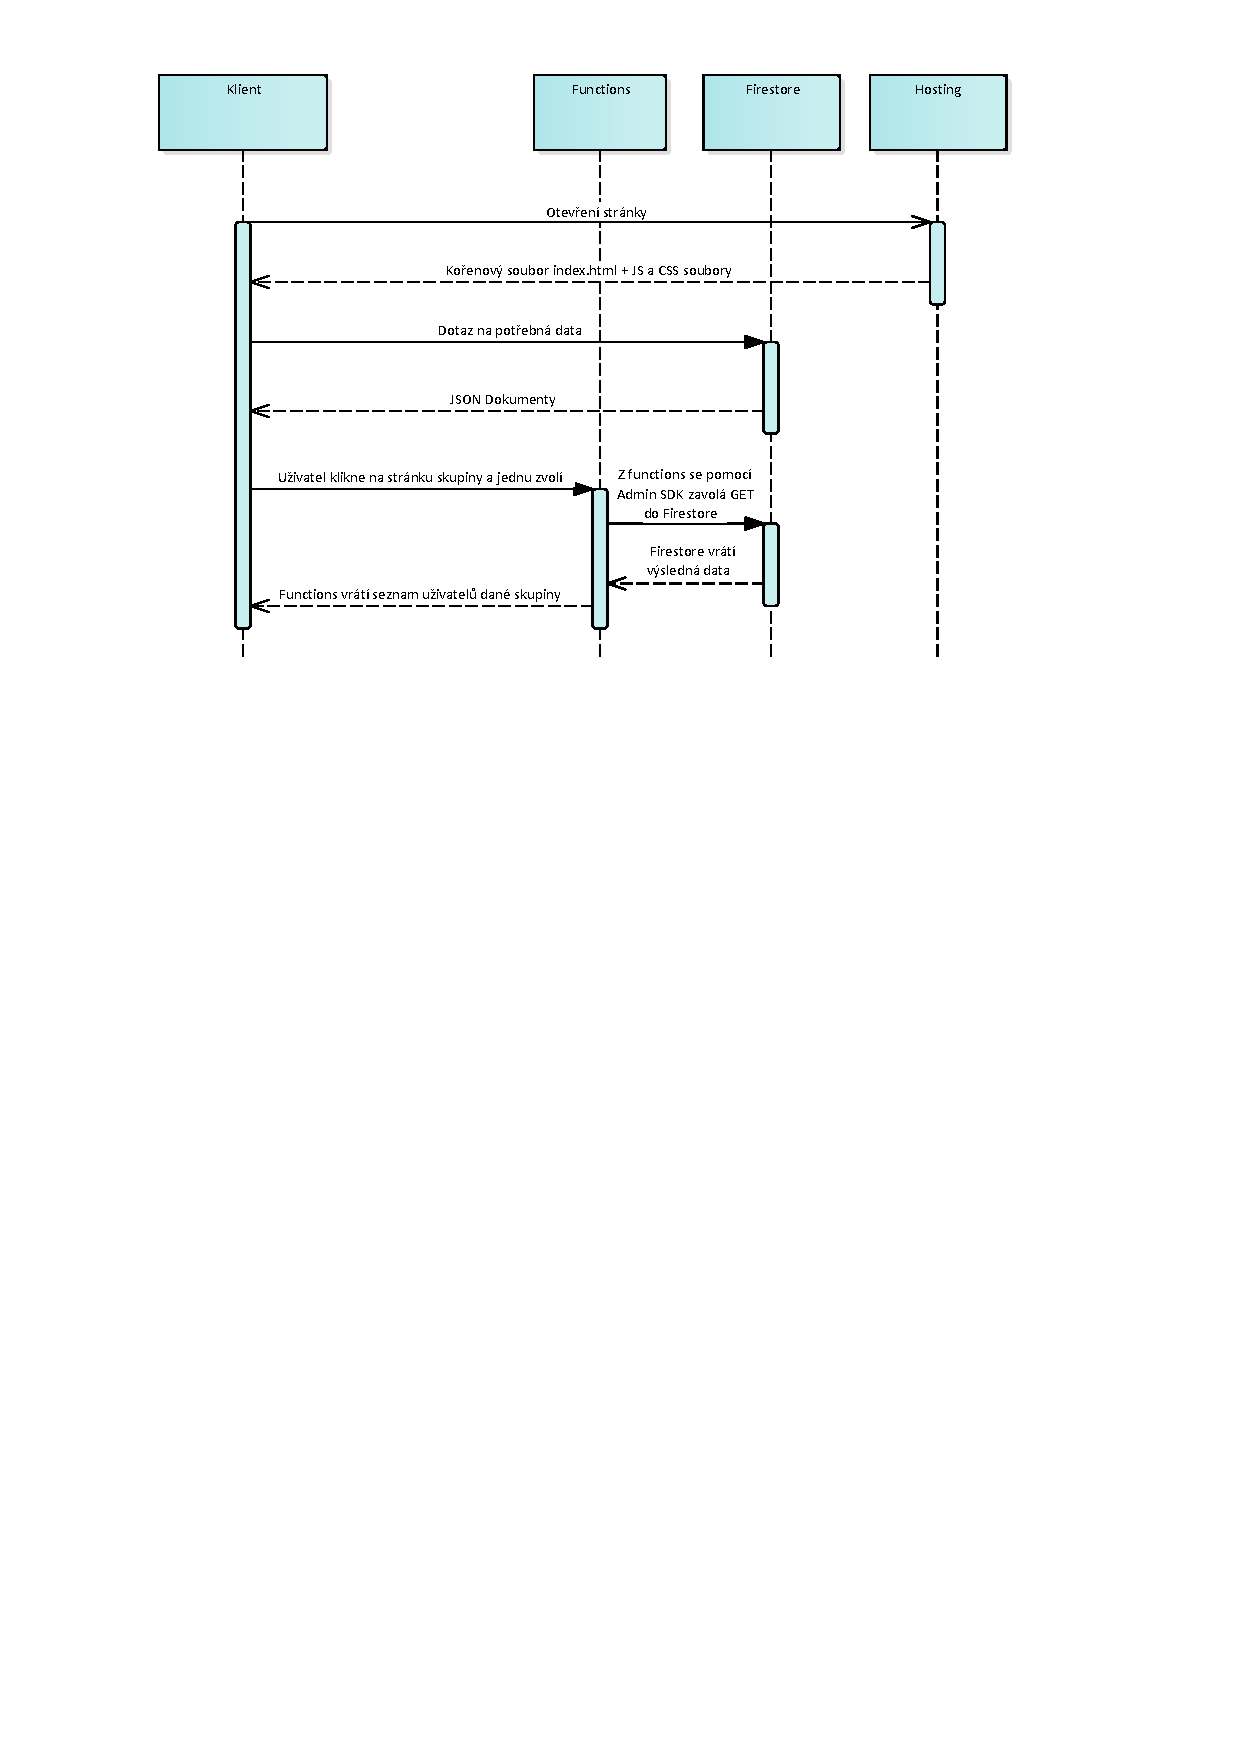
\includegraphics[width=\textwidth]{pdf/SPA-model}
    \caption{SPA Model} \label{picture:recipeo:spa-model}
\end{figure}

Jak je ve SPA diagramu vidět, některá data lze získat přímým přístupem do Firestore, ale jiná je nutné stáhnout z Functions.
Je to dané tím, že u některých dat není možné ošetřit jejich bezpečnost pomocí Firestore Rules a je tedy nutné k nim přistupovat
přes Functions, které má dostupné Admin SDK, tedy neomezený přístup k celé databázi. Data tak mohou být pro běžné uživatele nepřístupná,
ale pomocí volání cloudové funkce přímo z aplikace je možné je stáhnout. Také se dají data tímto způsobem předzpracovat, což může
být výhodné právě z hlediska bezpečnosti a k uživateli se tak nedostane nic co by nemělo.

\section{PWA}

Progresivní webová aplikace se snaží usnadnit vývoj standardních webových aplikací jako nativní aplikace pro mobilní telefony.
K tomu využívá \emph{service workers} a webové aplikační \emph{manifesty}. Aby se aplikace dala považovat za PWA, měla by
mít tyto vlastnosti~\cite{PWAAckee}.


\begin{itemize}
    \item Progresivní

    Je použitelná na starších prohlížečích s určitými omezeními, ale plně funkční na nejnovějších verzích prohlížečů.
    \item Responzivní

    Stránka je optimalizována pro všechny typy obrazovek (od nejmenších telefonů, přes notebooky až po velké PC monitory)
    \item Nezávislá na konektivitě

    Pomocí technologie \emph{service workers} je možné aplikaci využívat offline díky cachování
    \item App-like

    Aplikace vypadá jako nativní ačkoliv na pozadí je webová aplikace
    \item Aktuální

    Poskytují vždy aktuální verzi díky procesu update technologie \emph{service workers}
    \item Zabezpečená

    Výhradní použití HTTPS zamezí odposlouchávání či jiné manipulaci s přijímanými daty
    \item Znovuzapojení uživatele

    Je možné využít funkce push notifikace, která poté uživatele naláká zpět do aplikace \footnote{Tyto push notifikace z webového prohlížeče jsou již několik let běžnou
    záležitostí na systému Android, ale do iOS od společnosti Apple se dostaly teprve nedávno~\cite{PWANotifications}.}
    \item Instalovatelná

    Při přístupu na stránku je uživateli nabídnuto si aplikaci stáhnout, poté k ní může přistupovat jako k nativní aplikaci
    \item Odkazovatelná

    Dá se na ní jednoduše přistoupit pomocí URL bez nustnosti instalace
\end{itemize}

%! Author = Vojta
%! Date = 21.10.2021

\chapter{Nákup surovin}

\section{Možnosti}
Vedoucí práce již dříve používal aplikaci Zdravý stůl~\cite{ZdravyStul}. Tam bylo možné si jídlo objednat přes rohlik.cz (vložit do košíku).
Tudíž jsme chtěli tuto funkcionalitu zachovat a přidat možnosti jako například vytvoření objednávky u konkurence - kosik.cz
či zobrazení interaktivního nákupního listu.

\section{Komunikace s Rohlíkem a Košíkem}
Nejdříve jsme se rozhodli kontaktovat Rohlík. Po pár vyměněných e-mailech jsme obdrželi celou dokumentaci k jejich API,
které nám otevřelo spoutu možností i do budoucna. Například bychom mohli sledovat, jaké suroviny jsou právě ve slevě a
podle toho doporučovat jídla.

Od Košíku jsme dostali pozvání na schůzku, kde jsme si mohli prohlédnout i jejich kanceláře. Na schůzce jsme hned na začátku
zjistili, že API pro partnery narozdíl od Rohlíku ještě dostupné není (Rohlík na API pro partnery také teprve pracuje,
ale zatím jsme dostali přístup k API pro jejich aplikaci), ale už na něm pracují. Plánované období vydání je
první kvartál roku 2022. Pro jeho využití je však potřeba OAuth server, který zatím není dostupný. % TODO: Zjistit v lednu.
Jako alternativu jsme dohromady vymysleli link na přidání surovin přímo do košíku, ze kterého nakonec sešlo, protože jsme
poté objevili funkci \uv{Nákupní lístek}, kterou bychom mohli využít. Odeslali bychom seznam surovin a uživatel by si je poté
mohl vybrat přímo z nabídky na Košíku. Nakonec jsme zjistili, že by se Košíku hodilo rozrůst sbírku receptů a bylo by možné
pro uživatele naší aplikace nabínout jejich recepty Košíku, který by je následně odkoupil.


% % Do not forget to include Introduction
%---------------------------------------------------------------
\chapter{Ut enim ad minim veniam}
%---------------------------------------------------------------
\setcounter{page}{1}

\begin{chapterabstract}
	\lipsum[1]
\end{chapterabstract}

\lipsum[2][1-4]{} [1]

\lipsum[4]

%---------------------------------------------------------------
\section{Ut enim ad minim veniam}
%---------------------------------------------------------------

\lipsum[6-7]

\begin{figure}
\centering
%\includegraphics[scale=0.4]{pic/index}
\resizebox{\textwidth}{!}{
\begin{tikzpicture}[level/.style={sibling distance=60mm/#1}]
\node [circle,draw] (z){$n$}
  child {node [circle,draw] (a) {$\frac{n}{2}$}
    child {node [circle,draw] (b) {$\frac{n}{2^2}$}
      child {node {$\vdots$}
        child {node [circle,draw] (d) {$\frac{n}{2^k}$}}
        child {node [circle,draw] (e) {$\frac{n}{2^k}$}}
      }
      child {node {$\vdots$}}
    }
    child {node [circle,draw] (g) {$\frac{n}{2^2}$}
      child {node {$\vdots$}}
      child {node {$\vdots$}}
    }
  }
  child {node [circle,draw] (j) {$\frac{n}{2}$}
    child {node [circle,draw] (k) {$\frac{n}{2^2}$}
      child {node {$\vdots$}}
      child {node {$\vdots$}}
    }
  child {node [circle,draw] (l) {$\frac{n}{2^2}$}
    child {node {$\vdots$}}
    child {node (c){$\vdots$}
      child {node [circle,draw] (o) {$\frac{n}{2^k}$}}
      child {node [circle,draw] (p) {$\frac{n}{2^k}$}
        child [grow=right] {node (q) {$=$} edge from parent[draw=none]
          child [grow=right] {node (q) {$O_{k = \lg n}(n)$} edge from parent[draw=none]
            child [grow=up] {node (r) {$\vdots$} edge from parent[draw=none]
              child [grow=up] {node (s) {$O_2(n)$} edge from parent[draw=none]
                child [grow=up] {node (t) {$O_1(n)$} edge from parent[draw=none]
                  child [grow=up] {node (u) {$O_0(n)$} edge from parent[draw=none]}
                }
              }
            }
            child [grow=down] {node (v) {$O(n \cdot \lg n)$}edge from parent[draw=none]}
          }
        }
      }
    }
  }
};
\path (a) -- (j) node [midway] {+};
\path (b) -- (g) node [midway] {+};
\path (k) -- (l) node [midway] {+};
\path (k) -- (g) node [midway] {+};
\path (d) -- (e) node [midway] {+};
\path (o) -- (p) node [midway] {+};
\path (o) -- (e) node (x) [midway] {$\cdots$}
  child [grow=down] {
    node (y) {$O\left(\displaystyle\sum_{i = 0}^k 2^i \cdot \frac{n}{2^i}\right)$}
    edge from parent[draw=none]
  };
\path (q) -- (r) node [midway] {+};
\path (s) -- (r) node [midway] {+};
\path (s) -- (t) node [midway] {+};
\path (s) -- (l) node [midway] {=};
\path (t) -- (u) node [midway] {+};
\path (z) -- (u) node [midway] {=};
\path (j) -- (t) node [midway] {=};
\path (y) -- (x) node [midway] {$\Downarrow$};
\path (v) -- (y)
  node (w) [midway] {$O\left(\displaystyle\sum_{i = 0}^k n\right) = O(k \cdot n)$};
\path (q) -- (v) node [midway] {=};
\path (e) -- (x) node [midway] {+};
\path (o) -- (x) node [midway] {+};
\path (y) -- (w) node [midway] {$=$};
\path (v) -- (w) node [midway] {$\Leftrightarrow$};
\path (r) -- (c) node [midway] {$\cdots$};
\end{tikzpicture}}
\caption{~Lorem ipsum dolor sit amet}\label{img:index}
\end{figure}

%---------------------------------------------------------------
\section{Ut enim ad minim veniam}
%---------------------------------------------------------------

\lipsum[2-4]

%---------------------------------------------------------------
\subsection{Ut enim ad minim veniam}
%---------------------------------------------------------------

Curabitur ligula sapien, pulvinar a vestibulum quis, facilisis vel sapien. Duis condimentum augue id magna semper rutrum. Aliquam ornare wisi eu metus. Fusce aliquam vestibulum ipsum. Vivamus ac leo pretium faucibus\ref{img:index}.

\begin{itemize}
    \item Ut enim ad minim veniam, quis nostrud
    \item Ut enim ad minim
    \item Ut enim ad minim veniam, quis
    \begin{itemize}
        \item Ut enim ad
        \item Ut enim ad
        \begin{itemize}
            \item Ut enim
            \item Ut enim
            \begin{itemize}
            \item Ut enim
            \item Ut enim
        \end{itemize}
        \end{itemize}
    \end{itemize}
\end{itemize}

\section{Class aptent taciti}

\lipsum[2]

\subsection{Class aptent taciti}

\lipsum[6-7]

\begin{enumerate}
    \item Ut enim ad minim veniam, quis nostrud
    \item Ut enim ad minim
    \item Ut enim ad minim veniam, quis
    \begin{enumerate}
        \item Ut enim ad
        \item Ut enim ad
        \begin{enumerate}
            \item Ut enim
            \item Ut enim
            \begin{enumerate}
            \item Ut enim
            \item Ut enim
        \end{enumerate}
        \end{enumerate}
    \end{enumerate}
\end{enumerate}


%---------------------------------------------------------------
\section{Ut enim ad minim veniam, quis nostrud}
%---------------------------------------------------------------

Ut enim ad minim veniam, quis nostrud exercitation ullamco laboris nisi ut aliquip ex ea commodo consequat. Nulla non arcu lacinia neque faucibus fringilla. Vestibulum erat nulla, ullamcorper nec, rutrum non, nonummy ac, erat. Aliquam erat volutpat. Proin pede metus, vulputate nec, fermentum fringilla, vehicula vitae, justo.\footnote{Ut enim ad minim veniam, quis nostrud exercitation.} Etiam dictum tincidunt diam. In laoreet, magna id viverra tincidunt, sem odio bibendum justo, vel imperdiet sapien wisi sed libero. Nulla est. Maecenas fermentum, sem in pharetra pellentesque, velit turpis volutpat ante, in pharetra metus odio a lectus. Duis aute irure dolor in reprehenderit in voluptate velit esse cillum dolore eu fugiat nulla pariatur.

%\begin{lstlisting}[caption={~Zbytečný kód},label=list:8-6,captionpos=t,float,abovecaptionskip=-\medskipamount,belowcaptionskip=\medskipamount,language=C]
%    #include<stdio.h>
%    #include<iostream>
%    // A comment
%    int main(void)
%    {
%        printf("Hello World\n");
%        return 0;
%    }
%\end{lstlisting}

%%%%%%%%%%%%%%%%%%%%%%%%%%%%%%%%%
% alternative using package minted for source highlighting
% package minted requires execution with `-shell-escape'
% e.g., `xelatex -shell-escape ctufit-thesis.tex'
\begin{listing}
\caption{Zbytečný kód}\label{list:8-6}
\begin{minted}{C}
    #include<stdio.h>
    #include<iostream>
    // A comment
    int main(void)
    {
        printf("Hello World\n");
        return 0;
    }
\end{minted}
\end{listing}
% %%%%%%%%%%%%%%%%%%%%%%%%%%%%%%%%%
Nullam feugiat, turpis at pulvinar vulputate, erat libero tristique tellus, nec bibendum odio risus sit amet ante. Aenean id metus id velit ullamcorper pulvinar. Fusce wisi. Integer lacinia. Aliquam id dolor. Pellentesque pretium lectus id turpis. Suspendisse sagittis ultrices augue. In laoreet, magna id viverra tincidunt, sem odio bibendum justo, vel imperdiet sapien wisi sed libero. Sed ac dolor sit amet purus malesuada congue. \cite{Crochemore2002}

Class aptent taciti sociosqu ad litora torquent per conubia nostra, per inceptos hymenaeos. Fusce suscipit libero eget elit. Etiam dui sem, fermentum vitae, sagittis id, malesuada in, quam. Aliquam id dolor. Curabitur bibendum justo non orci. Duis viverra diam non justo. Curabitur ligula sapien, pulvinar a vestibulum quis, facilisis vel sapien. Duis condimentum augue id magna semper rutrum. Aliquam ornare wisi eu metus. Fusce aliquam vestibulum ipsum. Vivamus ac leo pretium faucibus. \cite{Motwani2014}

%---------------------------------------------------------------
\subsection{Ut enim ad minim veniam, quis nostrud}
%---------------------------------------------------------------

Ut enim ad minim veniam, quis nostrud exercitation ullamco laboris nisi ut aliquip ex ea commodo consequat. Nulla non arcu lacinia neque faucibus fringilla. Vestibulum erat nulla, ullamcorper nec, rutrum non, nonummy ac, erat. Aliquam erat volutpat. Proin pede metus, vulputate nec, fermentum fringilla, vehicula vitae, justo. Etiam dictum tincidunt diam. In laoreet, magna id viverra tincidunt, sem odio bibendum justo. \cite{Sestakova2018}

\begin{table}\centering
\caption[Příklad tabulky]{~Zadávání matematiky}\label{tab:matematika}
\begin{tabular}{l|l|c|c}
	Typ		& Prostředí		& \LaTeX{}ovská zkratka	& \TeX{}ovská zkratka	\tabularnewline \hline
 	Text		& \verb|math|		& \verb|\(...\)|	& \verb|$...$|	\tabularnewline \hline
 	Displayed	& \verb|displaymath|	& \verb|\[...\]|	& \verb|$$...$$|	\tabularnewline
\end{tabular}
\end{table}


Nulla est. Maecenas fermentum, sem in pharetra pellentesque, velit turpis volutpat ante, in pharetra metus odio a lectus. Duis aute irure dolor in reprehenderit in voluptate velit esse cillum dolore eu fugiat nulla pariatur. Nullam feugiat, turpis at pulvinar vulputate, erat libero tristique tellus, nec bibendum odio risus sit amet ante. Aenean id metus id velit ullamcorper pulvinar.

\subsubsection{Class aptent taciti}

\begin{definition}[Optional label]
Class aptent taciti sociosqu ad litora torquent per conubia nostra, per inceptos hymenaeos. Fusce suscipit libero eget elit. Etiam dui sem, fermentum vitae, sagittis id, malesuada in, quam. Aliquam id dolor. Curabitur bibendum justo non orci.
\end{definition}

\begin{example}
Class aptent taciti sociosqu ad litora torquent per conubia nostra, per inceptos hymenaeos. Fusce suscipit libero eget elit. Etiam dui sem, fermentum vitae, sagittis id, malesuada in, quam. Aliquam id dolor. Curabitur bibendum justo non orci.
\end{example}

\begin{theorem}
Class aptent taciti sociosqu ad litora torquent per conubia nostra, per inceptos hymenaeos. Fusce suscipit libero eget elit. Etiam dui sem, fermentum vitae, sagittis id, malesuada in, quam. Aliquam id dolor. Curabitur bibendum justo non orci.
\end{theorem}

\begin{proof}
Fusce suscipit libero eget elit. Etiam dui sem, fermentum vitae, sagittis id, malesuada in, quam. Aliquam id dolor. Curabitur bibendum justo non orci.
\end{proof}

\begin{corollary}
Fusce suscipit libero eget elit. Etiam dui sem, fermentum vitae, sagittis id, malesuada in, quam. Aliquam id dolor. Curabitur bibendum justo non orci.
\end{corollary}

\begin{proposition}
Fusce suscipit libero eget elit. Etiam dui sem, fermentum vitae, sagittis id, malesuada in, quam. Aliquam id dolor. Curabitur bibendum justo non orci.
\end{proposition}

\begin{note}
Fusce suscipit libero eget elit. Etiam dui sem, fermentum vitae, sagittis id, malesuada in, quam. Aliquam id dolor. Curabitur bibendum justo non orci.
\end{note}

\begin{remark}
Fusce suscipit libero eget elit. Etiam dui sem, fermentum vitae, sagittis id, malesuada in, quam. Aliquam id dolor. Curabitur bibendum justo non orci.
\end{remark}

\begin{lemma}
Class aptent taciti sociosqu ad litora torquent per conubia nostra, per inceptos hymenaeos. Fusce suscipit libero eget elit. Etiam dui sem, fermentum vitae, sagittis id, malesuada in, quam. Aliquam id dolor. Curabitur bibendum justo non orci.
\end{lemma}

\lipsum[1-2]

\subsection{Class aptent taciti sociosqu}

\lipsum[4-5]

%---------------------------------------------------------------
\chapter{Lorem ipsum}
%---------------------------------------------------------------

\begin{chapterabstract}
	Lorem ipsum dolor sit amet, consectetuer adipiscing elit. Curabitur sagittis hendrerit ante. Class aptent taciti sociosqu ad litora torquent per conubia nostra, per inceptos hymenaeos. Cras pede libero, dapibus nec, pretium sit amet, tempor quis. Sed vel lectus. Donec odio tempus molestie, porttitor ut, iaculis quis, sem. Cras pede libero, dapibus nec, pretium sit amet, tempor quis. Sed vel lectus.
\end{chapterabstract}

Lorem ipsum dolor sit amet, consectetuer adipiscing elit. Curabitur sagittis hendrerit ante. Class aptent taciti sociosqu ad litora torquent per conubia nostra, per inceptos hymenaeos. Cras pede libero, dapibus nec, pretium sit amet, tempor quis. Sed vel lectus. Donec odio tempus molestie, porttitor ut, iaculis quis, sem. Suspendisse sagittis ultrices augue. Donec ipsum massa, ullamcorper in, auctor et, scelerisque sed, est. In sem justo, commodo ut, suscipit at, pharetra vitae, orci. Pellentesque pretium lectus id turpis. \cite{Kopka2004}

\section{Donec odio tempus molestie}

\lipsum[2] \cite{def:1, def:2}

\subsection{Class aptent taciti}

\lipsum[2-3]

\begin{description}
\item[Kapitola 1] Lorem ipsum dolor sit amet, consectetuer adipiscing elit. Curabitur sagittis hendrerit ante. Class aptent taciti sociosqu ad litora torquent per conubia nostra, per inceptos hymenaeos. Cras pede libero, dapibus nec, pretium sit amet, tempor quis.

\item[Kapitola 2] Lorem ipsum dolor sit amet, consectetuer adipiscing elit. Curabitur sagittis hendrerit ante. Class aptent taciti sociosqu ad litora torquent per conubia nostra, per inceptos hymenaeos. Cras pede libero, dapibus nec, pretium sit amet, tempor quis.

\item[Kapitola 3] Lorem ipsum dolor sit amet, consectetuer adipiscing elit. Curabitur sagittis hendrerit ante. Class aptent taciti sociosqu ad litora torquent per conubia nostra, per inceptos hymenaeos. Cras pede libero, dapibus nec, pretium sit amet, tempor quis.

\item[Kapitola 4] Lorem ipsum dolor sit amet, consectetuer adipiscing elit. Curabitur sagittis hendrerit ante. Class aptent taciti sociosqu ad litora torquent per conubia nostra, per inceptos hymenaeos. Cras pede libero, dapibus nec, pretium sit amet, tempor quis.
\end{description}

\lipsum[2]

\section{Lorem ipsum dolor sit amet}

\lipsum[3-5]
 % include `examples.tex' from `text/' subdirectory

\appendix\appendixinit % do not remove these two commands

\chapter{Nějaká příloha}


Sem přijde to, co nepatří do hlavní části.
 % include `appendix.tex' from `text/' subdirectory

\backmatter % do not remove this command

\printbibliography % print out the BibLaTeX-generated bibliography list

\chapter{Obsah přiloženého média}
% TODO: Odstranit?

	\dirtree{%
		.1 readme.txt\DTcomment{stručný popis obsahu média}.
		.1 exe\DTcomment{adresář se spustitelnou formou implementace}.
		.1 src.
		.2 impl\DTcomment{zdrojové kódy implementace}.
		.2 thesis\DTcomment{zdrojová forma práce ve formátu \LaTeX{}}.
		.1 text\DTcomment{text práce}.
		.2 thesis.pdf\DTcomment{text práce ve formátu PDF}.
	}
 % include `medium.tex' from `text/' subdirectory

\end{document}
